%%%%%%%%%%%%%%%%%%%%%%%%%%%%%%%%%%%%%%%%%
% Stylish Article
% LaTeX Template
% Version 2.1 (1/10/15)
%
% This template has been downloaded from:
% http://www.LaTeXTemplates.com
%
% Original author:
% Mathias Legrand (legrand.mathias@gmail.com) 
% With extensive modifications by:
% Vel (vel@latextemplates.com)
%
% License:
% CC BY-NC-SA 3.0 (http://creativecommons.org/licenses/by-nc-sa/3.0/)
%
%%%%%%%%%%%%%%%%%%%%%%%%%%%%%%%%%%%%%%%%%

%----------------------------------------------------------------------------------------
%	PACKAGES AND OTHER DOCUMENT CONFIGURATIONS
%----------------------------------------------------------------------------------------

\documentclass[fleqn,24pt]{SelfArx} % Document font size and equations flushed left

\usepackage[english]{babel} % Specify a different language here - english by default

\usepackage [autostyle, english = american]{csquotes}
\MakeOuterQuote{"}
%----------------------------------------------------------------------------------------
%	COLUMNS
%----------------------------------------------------------------------------------------

\setlength{\columnsep}{0.55cm} % Distance between the two columns of text
\setlength{\fboxrule}{0.75pt} % Width of the border around the abstract

%----------------------------------------------------------------------------------------
%	COLORS
%----------------------------------------------------------------------------------------

\definecolor{color1}{RGB}{0,0,90} % Color of the article title and sections
\definecolor{color2}{RGB}{0,20,20} % Color of the boxes behind the abstract and headings

%----------------------------------------------------------------------------------------
%	HYPERLINKS
%----------------------------------------------------------------------------------------

\usepackage{hyperref} % Required for hyperlinks
\graphicspath{ {images/} }
\hypersetup{hidelinks,colorlinks,breaklinks=true,urlcolor=color2,citecolor=color1,linkcolor=color1,bookmarksopen=false,pdftitle={Title},pdfauthor={Author}}

%----------------------------------------------------------------------------------------
%	ARTICLE INFORMATION
%----------------------------------------------------------------------------------------

\JournalInfo{20 February 2016} % Journal information
\Archive{} % Additional notes (e.g. copyright, DOI, review/research article)

\PaperTitle{UBC CPSC 416 Distributed Systems: Project Proposal} % Article title

\Authors{Alcuaz, Ito Franchilo Mikael\textsuperscript{1}
| Aziz, Shariq\textsuperscript{2}
| Ko, Mimi\textsuperscript{3}
| Musa, Abrar\textsuperscript{4}
} % Authors
\affiliation{\textsuperscript{1}\textit{y9u8, ialcuaz@alumni.ubc.ca}} % Author affiliation
\affiliation{\textsuperscript{2}\textit{i2u9a, shariqazz15@gmail.com}} % Author affiliation
\affiliation{\textsuperscript{3}\textit{o3d7, mimi@dbzmail.com}} % Author affiliation
\affiliation{\textsuperscript{4}\textit{i1u9a, abrar.musa.89@gmail.com}} % Author affiliation

\Keywords{} % Keywords - if you don't want any simply remove all the text between the curly brackets
\newcommand{\keywordname}{Keywords} % Defines the keywords heading name

%----------------------------------------------------------------------------------------
%	ABSTRACT
%----------------------------------------------------------------------------------------

\Abstract{

Media streaming refers to the constant delivery of time-ordered multimedia content from a server to a client. It is an attractive option as opposed to conventional file transfer methodologies as it provides instant access for the end user and is quite flexible -- a user doesn't have to download the entire file beforehand as was traditionally done in the past, and can interact with the data as it arrives.
Naturally, such a system demands a high bandwidth connection and so works more effectively for users on faster internet networks. This proposal serves as an outline for a possible solution to this key shortcoming by de-centralizing the server-client model through the use of peer-to-peer (P2P) stream networking.
}

%----------------------------------------------------------------------------------------

\begin{document}

\flushbottom % Makes all text pages the same height

\maketitle % Print the title and abstract box

\tableofcontents

\thispagestyle{empty} % Removes page numbering from the first page

%----------------------------------------------------------------------------------------
%	ARTICLE CONTENTS
%----------------------------------------------------------------------------------------

\section{Introduction} % The \section*{} command stops section numbering

A P2P implementation of a media streaming system alleviates some of the bandwidth requirements due to the fact that content is distributed over several streams rather than over one singular server. Usually the content is multicasted from a server to some number of clients which has requested the stream; YouTube makes use of this notion by deploying multiple content delivery networks (CDNs) which distribute the content by demand; the video content is streamed over a single connection, and as such, demands a high bandwidth for maximum playability. 

The idea behind using P2P streaming is to make the system more scalable -- as the number of clients increase, so do the number of potential peers which can now act as a source, and thus share part of the bandwidth requirements. It does this by making the data available to other clients who also requested the stream, similar to how P2P BitTorrent file sharing works. The server and clients therefore together form a network of media streams.

Such a system, however, must preserve an invariant trait: clients must be able to connect and disconnect at will -- it must be able to discover the parent server through a given URL and leave at any point in time; client behaviour is inherently unpredictable especially in P2P systems which presents numerous complications. There must also exist logic to decide which clients copy parts of the stream, and application level functionality to allow a client to reject P2P connections (similar to rejecting seeding in BitTorrent applications).During the early 2000s, studies have been done on the usage of overlay systems for multicast applications. These systems were conventionally implemented at the end systems.

A few popular P2P implementations are PeerCast (2004) \cite{1}, SplitStream (2003), SCRIBE (2002), and Pastry (2001) \cite{3}. The first in this list will be examined primarily and used as a model for this group's implementation which will use the Go programming language. 

\begin{figure}[!htb]
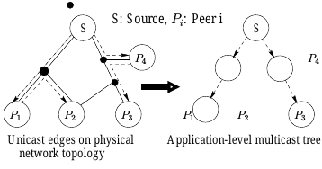
\includegraphics{Selection_148.png}
\caption{\label{family}A multicast tree.}
\label{1}
\end{figure}

\section{Implementation Strategy}

\subsection{Software engineering practices}
To follow good industry practices, this group will probably follow test driven development (TDD) and SCRUM methods throughout the development of the project, so that feature implementation is planned and executed with minimal risk. 

\subsection{Construction of a single, centralized server, and requesting clients}
This is the base case of the problem statement and should be implemented first and foremost. A server with a dummy file will be set up and a client will connect and stream the file to completion through a connection. To closely mimic standard video transferring protocols, a TCP connection will be first set up between the two on the initial handshake phase, and then use UDP packets to stream the data. It is critical that the packets be time-ordered. The server should be able to handle an arbitrary number of clients, and detect disconnections and failures. The dissemination tree of a basic multicast overlay system is thus constructed at this step.

\subsection{Stream forwarding policies}
Clients must be able to replicate the stream or parts of it from the server. An algorithm to decide where the server forwards its stream will also be implemented; the amount of forwarding must scale proportional to the number of connected clients. As above, failures and disconnects must be detected, such as the case of a replicated stream that is lost. In this step the basic join/leave/stream transfer policies as outlined in SCRIBE/Pastry will be implemented.

\subsection{P2P streaming, edge case failures, and application level functionality}
Clients will then be able to stream the data through other clients; there must exist an algorithm to decide when to do so, and the client which is streaming data to another client must communicate with the server to avoid data redundancy. This is the point in the project where the discussion, edge cases, and some of the specific heuristics discussed in \cite{1} and \cite{2} will come into fruition, and as such, will likely take significantly more time than the other segments. It would also be a nice plus to implement a feature which allows a client to prevent itself from acting as a source.

\subsection{Project deployment and extras}
In this section the GUI will be implemented, and the project will be hosted on a free website, possibly Heroku. It is hoped that any user can then upload multimedia content to some centralized server (maybe their machines can also act as servers ?), of which other users can then stream using the algorithms implemented above.

\section{Project Timeline}

To allow as much time as possible for polishing, debugging, and unforeseeable events, the meat of sections 2.2 - 2.4 should be completed on, or 1-2 weeks after Mar. 18, which corresponds to the project status meeting date. Step 2.2 most definitely needs to be finished as soon as possible within the next few weeks and shouldn't take as long as the subsequent steps.

\section{SWOT Analysis}

\subsection{Strengths}
There is a wealth of resources available on P2P streaming and established solutions which would serve to simplify the design and implementation process. The P2P system self scales as more nodes join, which is at the heart of distributed systems. PeerCast and other similar systems are well studied with respect to their advantages, drawbacks, and vulnerabilities.

\subsection{Weaknesses}
The system will be difficult to test and complicated to build due to the replication procedures, P2P links, unpredictability of node behaviour, etc. Performance will also be difficult to optimize as opposed to unicast-esque server-client implementations.

\subsection{Opportunities}
The Go programming language was created to specifically build distributed systems. As was seen in the class assignments, standard networking procedures are fairly straightforward to implement using this language. This project can be easily integrated with newer ideas r.e. media streaming.

\subsection{Threats}
The Go programming language is fairly new which makes well established solutions to specific problems harder to come by than other languages. Furthermore, the members of this group have not had experience with it prior to taking this course, and as such, the best practices and idioms that come with this language will not come as intuitively. 

\section{Conclusion}

A possible solution to the drawback of the centralized client-server model in media streaming can be found through the use of a multicasted, P2P network. This is achieved by sharing the bandwidth requirements across several disjoint nodes which serve to forward the data stream among themselves, not over one singular connection. Such a system is complicated to build however, and gives rise to its own set of disadvantages.

\phantomsection
\bibliographystyle{unsrt}
\bibliography{sample}

%------------------------------------------------

\end{document}